% Capa
\imprimircapa


% Folha de rosto
% o * indica que haverá a ficha bibliográfica
\imprimirfolhaderosto*

% Inserir a ficha bibliografica
% http://ficha.bu.ufsc.br/
\begin{fichacatalografica}
	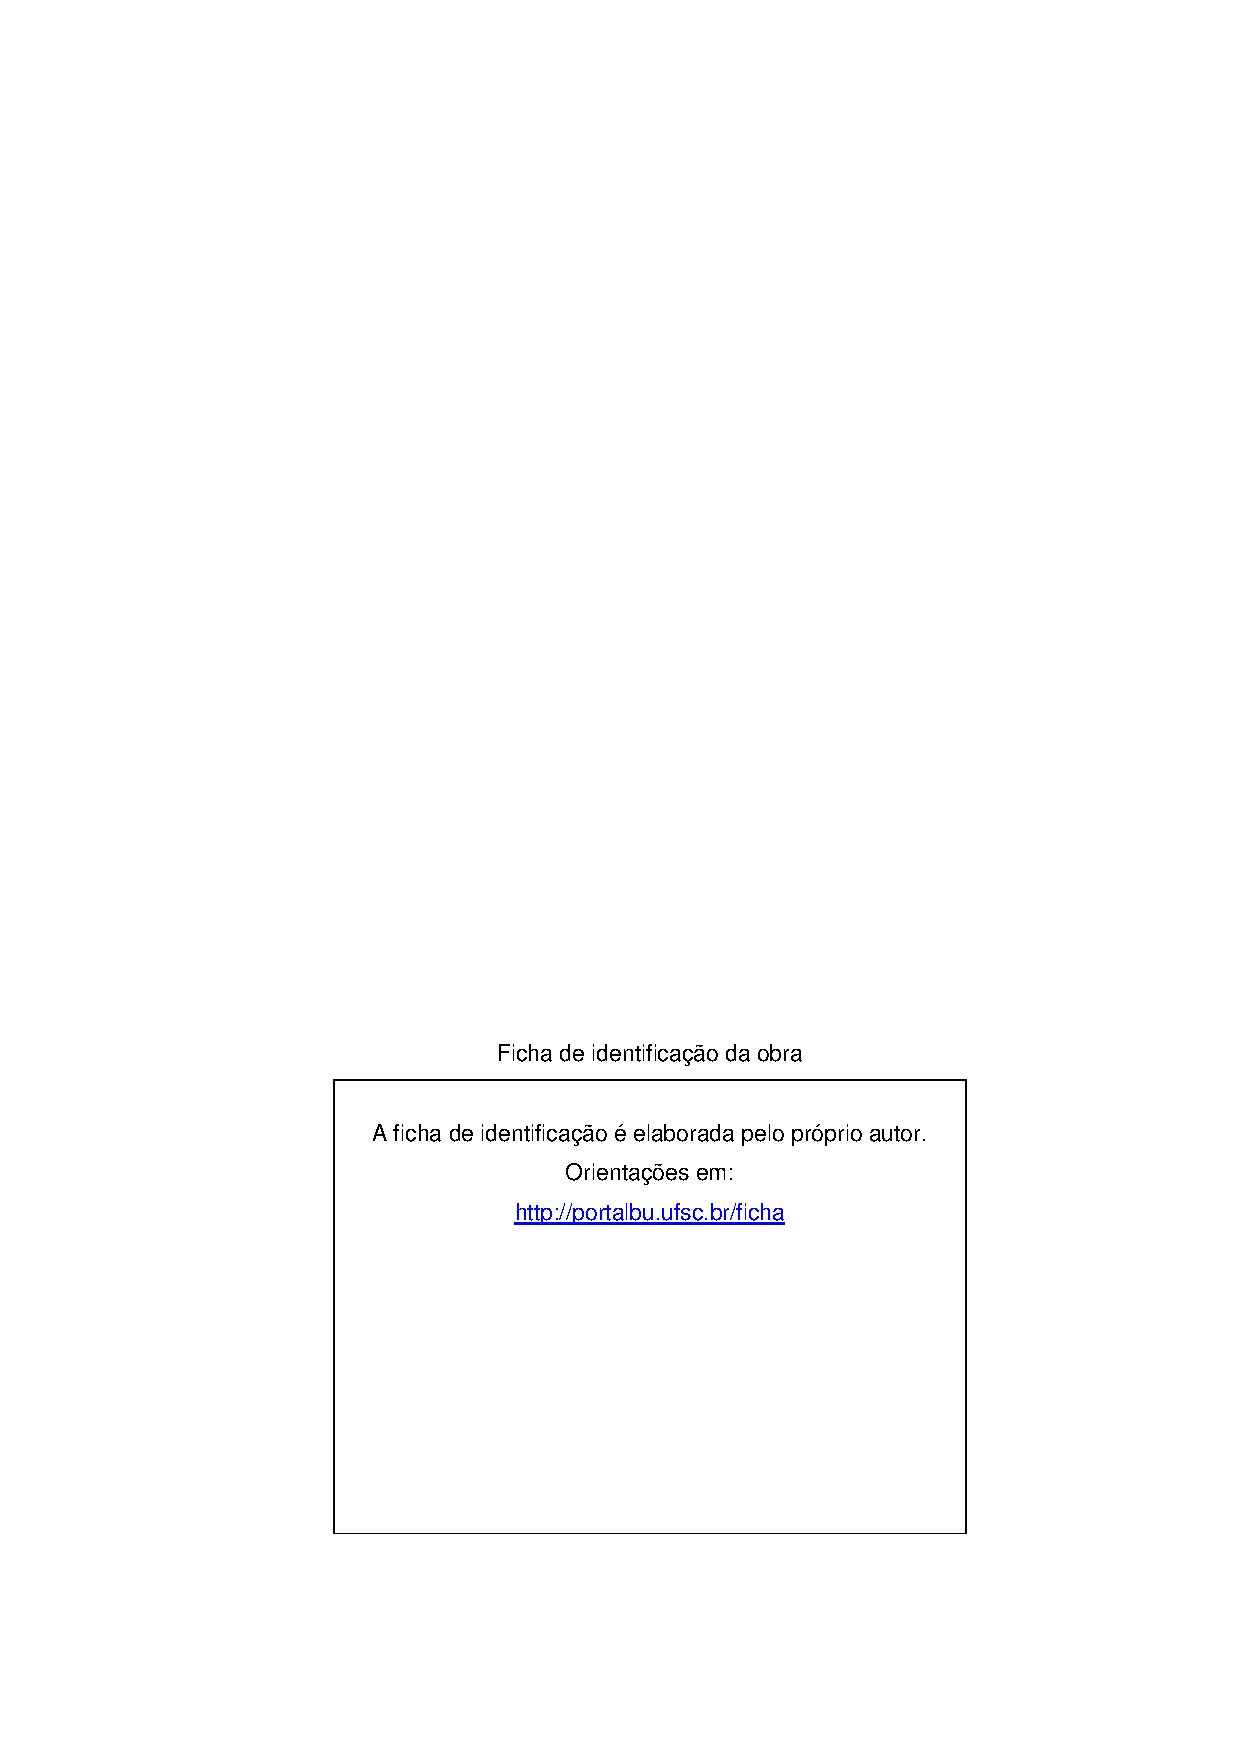
\includepdf{pre_textual/ficha_catalografica.pdf}
\end{fichacatalografica}

% Inserir folha de aprovação
\begin{folhadeaprovacao}
	\OnehalfSpacing
	\centering
	\imprimirautor\\%
	\vspace{24pt}		
	\textbf{\imprimirtitulo}%
	\ifnotempty{\imprimirsubtitulo}{:~\imprimirsubtitulo}\\%
	%		\vspace*{31.5pt}%3\baselineskip
	\vspace*{\baselineskip}
	%\begin{minipage}{\textwidth}
	Este Trabalho de Conclusão de Curso foi julgado adequado para obtenção do Título de ``\imprimirformacao'' e aprovado em sua forma final pelo Curso de Graduação em Engenharia de Controle e Automação.\\
	\vspace{12pt}
	\imprimirlocal, \imprimirdia~de~\imprimirmes~de~\imprimirano.\\
	
	\vspace*{18pt}
	\textbf{Banca Examinadora:}\\
	
	\vspace*{24pt}
	\assinatura{\OnehalfSpacing \imprimirbancanomea}
	\vspace{6pt}
	\imprimirbancainsta\\
	
	\vspace*{24pt}
	\assinatura{\OnehalfSpacing \imprimirbancanomeb}
	\vspace{6pt}
	\imprimirbancainstb\\
	
	\vspace*{24pt}
	\assinatura{\OnehalfSpacing \imprimirbancanomec}
	\vspace{6pt}
	\imprimirbancainstc\\
	
\end{folhadeaprovacao}

% Dedicatória
\ifnotempty{\imprimirdedicatoriatcc}{
\begin{dedicatoria}
	\vspace*{\fill}
	\noindent
	\begin{adjustwidth*}{}{7.5cm} 
		\textit{\imprimirdedicatoriatcc}
	\end{adjustwidth*}
\end{dedicatoria}
}

% Agradecimentos
\ifnotempty{\imprimiragradecimentostcc}{
\begin{agradecimentos}
	\imprimiragradecimentostcc
\end{agradecimentos}
}

% Epígrafe
\ifnotempty{\imprimirepigrafetcc}{
\begin{epigrafe}
	\vspace*{\fill}
        \noindent
	\begin{adjustwidth*}{}{7.5cm}
	       \textit{\imprimirepigrafetcc}
        \end{adjustwidth*}
\end{epigrafe}
}


% Resumo
\setlength{\absparsep}{18pt} % ajusta o espaçamento dos parágrafos do resumo
\begin{resumo}
	\SingleSpacing
	\imprimirresumotcc
	
	\textbf{Palavras-chave}: \imprimirpalavraschave
\end{resumo}

% Abstract
\begin{resumo}[Abstract]
	\SingleSpacing
	\imprimirabstracttcc
		
	\textbf{Keywords}: \imprimirkeywords
\end{resumo}


{%hidelinks
	\hypersetup{hidelinks}
	
	% inserir lista de figuras
	\pdfbookmark[0]{\listfigurename}{lof}
	\listoffigures*
	\cleardoublepage
	
	% inserir lista de quadros
	\ifnotempty{\verificaquadros}{
		\pdfbookmark[0]{\listofquadrosname}{loq}
		\listofquadros*
		\cleardoublepage
	}
	
	% inserir lista de tabelas
	\pdfbookmark[0]{\listtablename}{lot}
	\listoftables*
	\cleardoublepage
	
	% inserir lista de abreviaturas e siglas (devem ser declarados no preambulo)
	\ifnotempty{\verificasiglas}{
	\imprimirlistadesiglas
	}
	
	% inserir lista de símbolos (devem ser declarados no preambulo)
	\ifnotempty{\verificasimbolos}{
	\imprimirlistadesimbolos
	}
	
	% inserir o sumario
	\pdfbookmark[0]{\contentsname}{toc}
	\tableofcontents*
	\cleardoublepage
	
}%hidelinks